\chapter{Example}
\label{Example}

A citatation goes like this~\cite{latex}

\begin{figure}
\centering
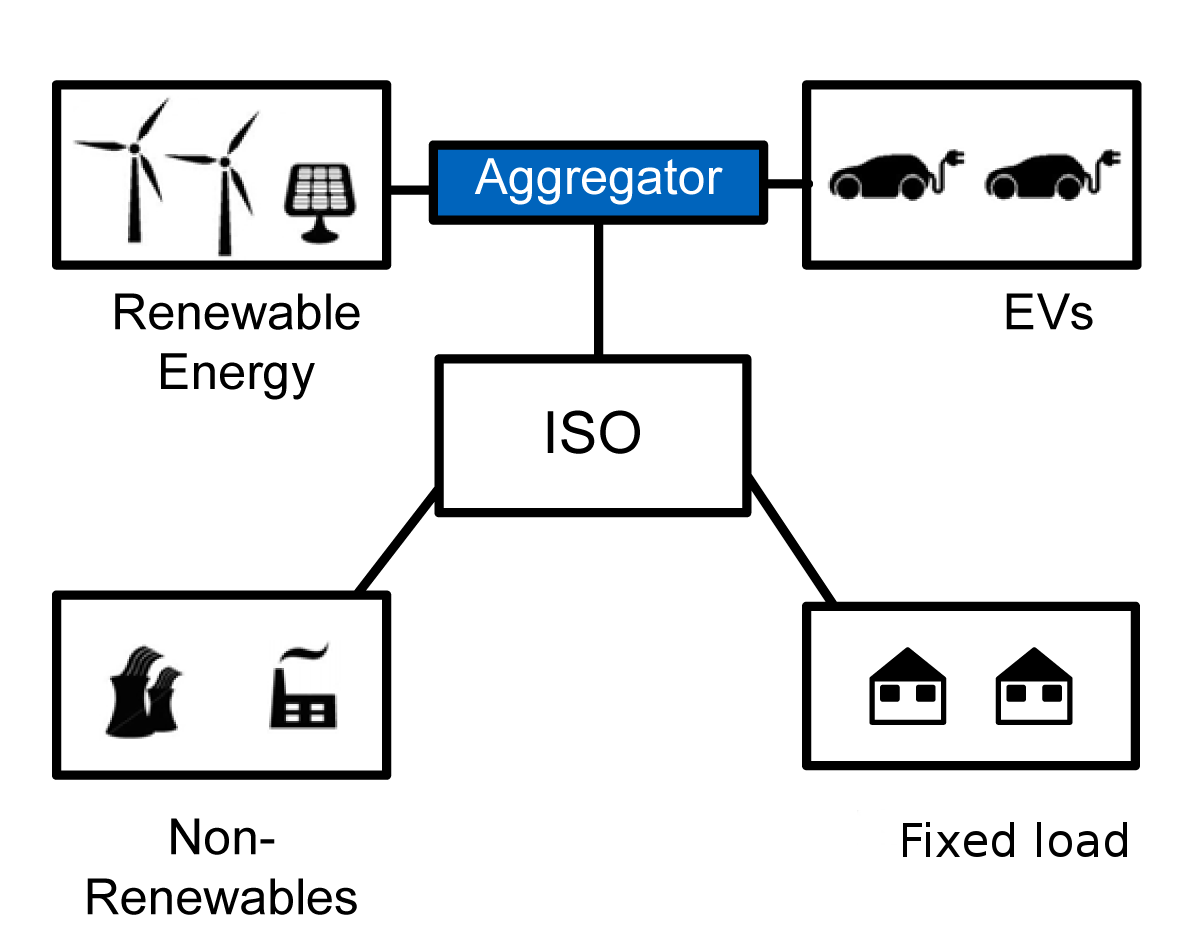
\includegraphics[width=0.8\linewidth]{figures/DirectCoupling}
\caption[Short caption for List of Figures]{Long caption. Displayed below the figure}
\label{fig:DirectCoupling}
\end{figure}

\begin{lstlisting}[language=java, basicstyle=\tiny, frame=single,	stringstyle=\color{red}, backgroundcolor=\color{Gray}, keywordstyle=\color{blue}, stringstyle=\color{red},commentstyle=\color{green},numbers=left, tabsize=2, label=lst:ev, caption={Implementation of Electric Vehicle for OVF.}, breaklines=true, captionpos=b]
public class OVF_EV extends ControllableDevice {
	public static final double EV_THRESHOLD = 0.001;
  private DopsVector value;
  private double requiredEnergy;
  private double[] drivingProfile; 	
  private double lowerChargingBound = 0;
  private double upperChargingBound = 4;

  public void initialize(File file) {
    MatFileReader mfr = new MatFileReader(file);
    MLDouble driveP = (MLDouble) mfr.getMLArray("d"); // driving profile
    drivingProfile = MatrixUtil.getFirstRow(driveP.getArray(), driveP.getN());
    MLDouble requiredE = (MLDouble) mfr.getMLArray("R"); // required energy
    requiredEnergy = requiredE.getArray()[0][0];
    value = new DopsVector(0);
  }

  public DopsVector getValue() {
    return value;
  }	
}
\end{lstlisting}
